% %开头表示注释

% 请看右下角你的编码格式是否为UTF-8或UTF-8 without BOM
% 写好后点击上方的编译, 选择使用XeLaTeX编译

% 这表示文档类为beamer(幻灯片)
\documentclass{beamer}
% 这表示这个幻灯片使用的主题为 Warsaw
\usetheme{Warsaw}
% 常用的一些包，不用动，有需要的再往后加就行
%\usepackage{mathrsfs}
%\usepackage[T1]{fontenc}
\usepackage{charter}
\usepackage{tikz}
\usepackage[nocap]{ctex}
\usepackage[english]{babel}
\usepackage{latexsym}
\usepackage[all]{xy}
\usepackage{graphics}
\usepackage{graphicx}
\usepackage{amssymb}
\usepackage{amsmath}
\usepackage{color}
\usepackage{subfigure}
\usepackage{mathrsfs}
\usefonttheme[onlymath]{serif}

% 定义缩写
% 整数环，使用 $\BZ$ 表示即可; 有理数、实数、复数、有限域类似.
% \mathbb为空心体
\newcommand{\BZ}{\mathbb{Z}}
\newcommand{\BQ}{\mathbb{Q}}
\newcommand{\BR}{\mathbb{R}}
\newcommand{\BC}{\mathbb{C}}
\newcommand{\BF}{\mathbb{F}}
% 线性映射可以用花体
\newcommand{\CF}{\mathcal{F}}
\newcommand{\CA}{\mathcal{A}}
\newcommand{\CB}{\mathcal{B}}
\newcommand{\CL}{\mathcal{L}}
\newcommand{\ch}{\mathrm{char}\;}
% 箭头
\newcommand{\ra}{\rightarrow}
\newcommand\lra{\longrightarrow}
% 单射
\newcommand\inj{\hookrightarrow}
% 满射
\newcommand\surj{\twoheadrightarrow}
% 带上标的箭头
\newcommand\sto[1]{\stackrel{#1}{\longrightarrow}}
% 同构于
\newcommand\simto{\sto{\sim}}
% 映射到
\newcommand\lto{\longmapsto}
% 上划线
\newcommand\ov{\overline}
% 下划线
\newcommand\ul{\underline}
% 花epsilon
\newcommand\vare{\varepsilon}
% 花phi
\newcommand\varp{\varphi}
% 推出
\newcommand\Ra{\Longrightarrow}
\newcommand\LRa{\Longleftrightarrow}
% 极限
\newcommand\ilim{\varinjlim\limits}
\newcommand\plim{\varprojlim\limits}
% 1/2
\newcommand\half{\frac{1}{2}}
% 双竖线
\newcommand\mmid{\parallel}
% 映射的缩写
\newcommand{\fct}[4]{\begin{split}#1&\lra #2\\#3&\lto #4\end{split}}


% 定理环境
\newtheorem{theoremA}[theorem]{Theorem~A}
\newtheorem{theoremB}[theorem]{Theorem~B}
\newtheorem{proposition}[theorem]{Proposition}
\newtheorem{conjecture}[theorem]{Conjecture}
\theoremstyle{remark}
\newtheorem{remark}[theorem]{Remark}
\numberwithin{equation}{section}

\def\baselinestretch{1}
\setlength{\parskip}{3mm}

% 正文开始
\begin{document}
% 标题
\title{Research Project on Linear Algebra}
% 作者
\author[S. Zhang \& S. Li]{San Zhang (张三), 2021000114\\
Si Li (李四), 2021000514
}
% 日期
\date{August 10$^\text{th}$, 2021}

% 封面页
\frame{\titlepage}

% 新的一页
\begin{frame}
\section{Statement}
% 居中环境
\begin{center}
\textcolor{blue}{ % 蓝色, LaTeX 中换行仅相当于一个空格
	\huge{ % 巨大 Huge huge Large large 
		\bfseries Statement %加粗
	}
}
\end{center}

The main results of our research project are: 
\begin{theoremA}\label{thm:A}% 标记用于引用
The conjugate classes of the solution of
	\[A^k=I_n\] % 行间公式，单独一行; ^表示上标, 
in $M_n(F)$ is \dots. % $..$ 为数学环境(行内公式); _表示下标
\end{theoremA}
\end{frame}
% 这一页结束


\begin{frame}
\begin{theoremB}\label{thm:B}% 标记用于引用
The ring homomorphisms of
	\[U_n(F)\to F[t]\]
are
\begin{enumerate}
\item $g(A)=\cdots$, where $A=(a_{ij})$; % 超过一个字符的上下标需要用大括号圈起来
\item for $i=1,\dots,n$, $f_i(A)=\cdots$, where $A=(a_{ij})$.
\end{enumerate}
Here we write $A=(a_{ij})\in U_n(F)$.
\end{theoremB}
\end{frame}
% 这一页结束


\begin{frame}
\section{Proof of Theorem~A}
% 居中环境
\begin{center}
\textcolor{red}{\Large{\bfseries Proof of Theorem~A}}
\end{center}
Let $F$ be a field with $\ch F=0$.
Let $A$ be a matrix in $M_{m,n}(F)$.

% 空白行才表示真的分段
Denote by $B=A^2$.
Denote by $S$ the set
	\[
		\{1,2,3,\dots\} % \{..\}表示真正的大括号, \dots 省略号
	\]
Let $f$ be a $F$-linear map
	\[\fct{f:V}{W}{v}{w.}\]% 包括箭头左边、右边，映射到的左边和右边四个部分

\end{frame}


\begin{frame}
Denote by
	\[A=\begin{pmatrix}
	1& 2& \cdots & n\\
	2& 3& \cdots & 1\\
	\vdots& \vdots & \ddots &\vdots\\
	n& 1&\cdots& n-1
	\end{pmatrix},
		\quad %短分割	
	B=\left[\begin{matrix}
	a_{11}& a_{12}& \cdots & a_{1n}\\
	a_{21}& a_{22}& \cdots & a_{2n}\\
	\vdots& \vdots & \ddots &\vdots\\
	a_{m1}& a_{m2}&\cdots& a_{m,n}
	\end{matrix}\right].\]
	
	\[C=\begin{bmatrix}
	1& 2& \cdots & n\\
	 & 1& \cdots & n-1\\
	& & \ddots &\vdots\\
	& && 1
	\end{bmatrix},
		\qquad % 稍长分割
	D=\begin{vmatrix}
	1& 2& \cdots & n\\
	2& 3& \cdots & 1\\
	\vdots& \vdots & \ddots &\vdots\\
	n& 1&\cdots& n-1
	\end{vmatrix}=?\]

\pause
Vector is a kind of special matrix.
\end{frame}


\begin{frame}
\begin{center}
% 插图
\begin{figure}
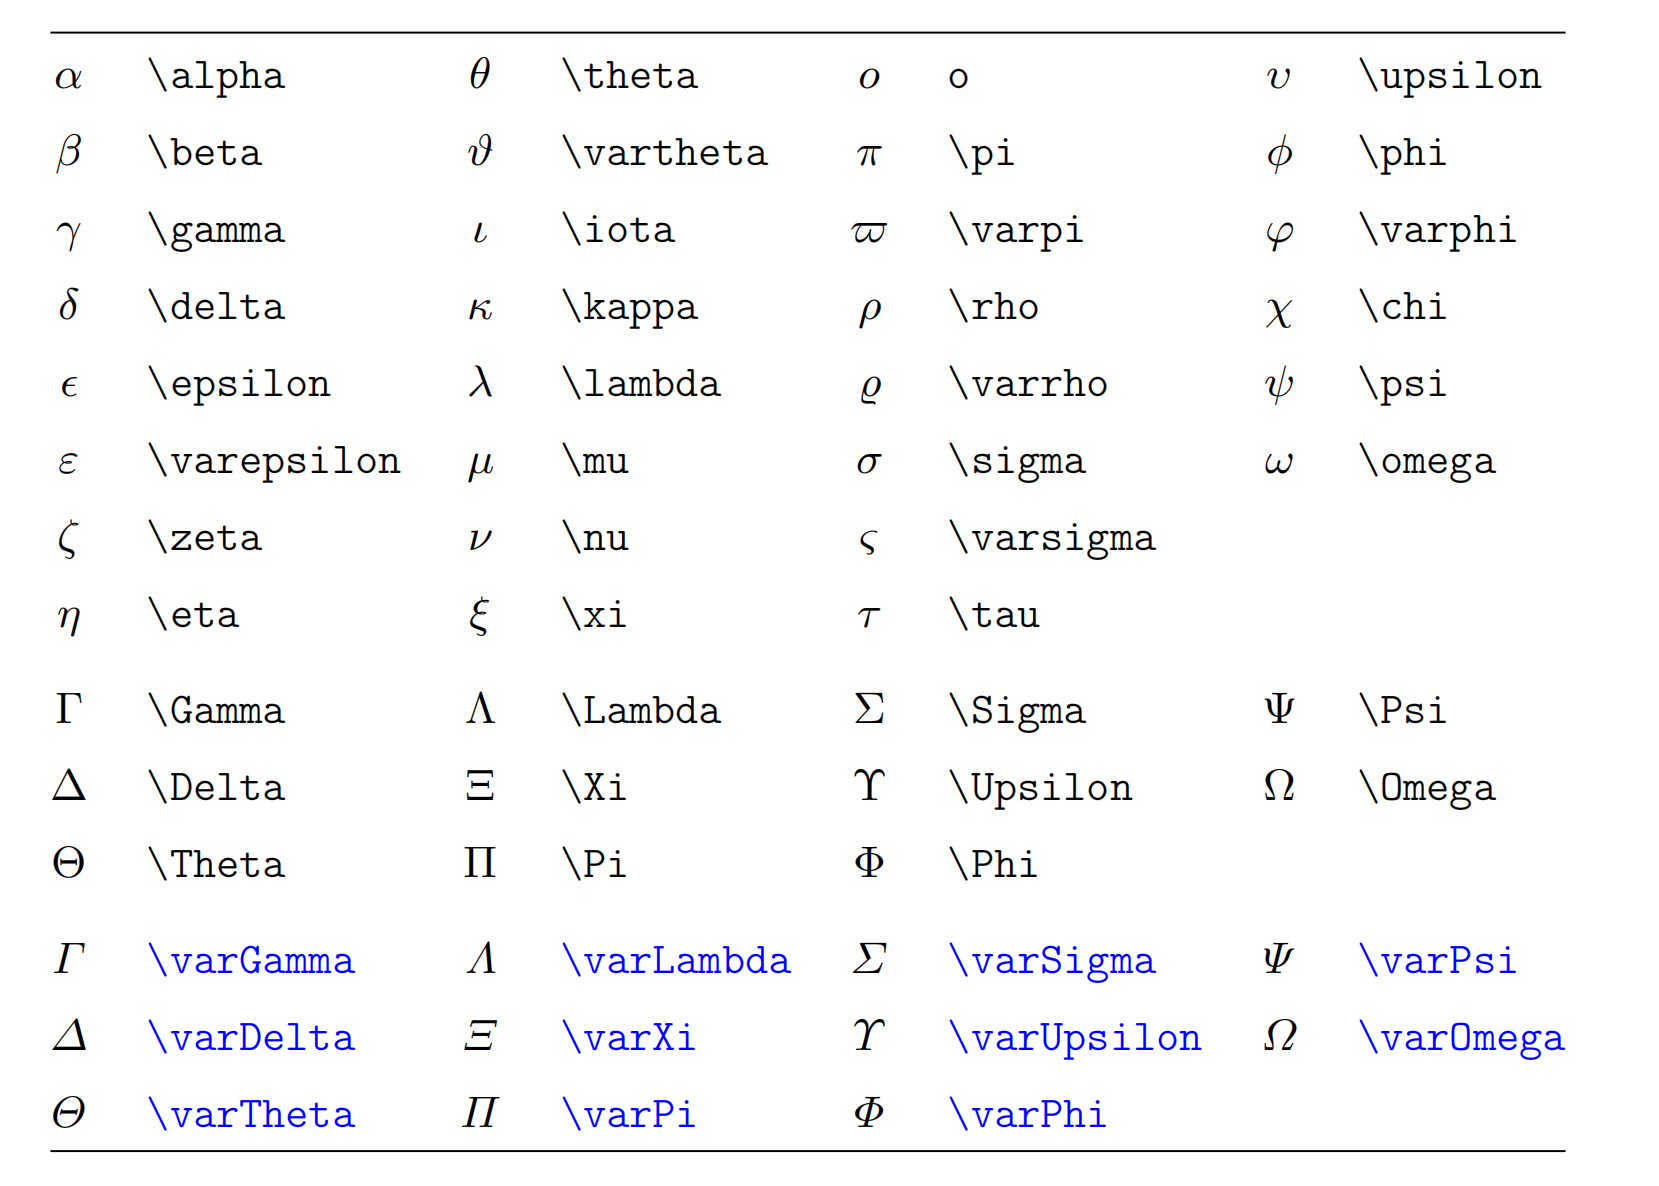
\includegraphics[height=7cm]{photo/greek.png}
\end{figure}
\end{center}
\end{frame}

\begin{frame}
See \ul{lshort.pdf} Chapter~4 for more symbols.

\begin{center}
\begin{figure}
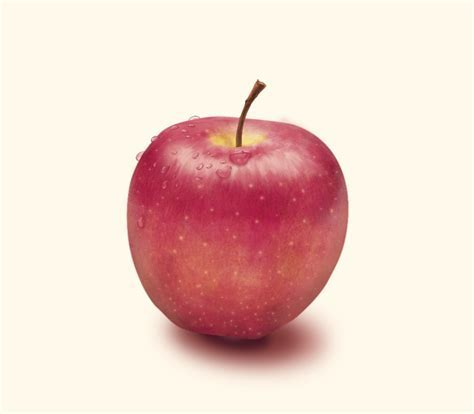
\includegraphics[height=3cm]{photo/apple.jpg}
\caption{An apple}
\end{figure}
\end{center}
\end{frame}


\begin{frame}

$\det, \mathrm{sgn}, \ov{fg}, \oplus, \times, \pm, \mp, \le, \ge, \simto, \cong, \in, \ni, \subset, \supset, \subseteq, \subsetneq, \cup,\cap,\int,\iint,\iiint,\Ra,\LRa, \hbar,\nabla$. \pause %幻灯片会在这里停留等待翻页
\[
\lim_{n\ra\infty}a_n=a,\quad
\ilim_{n\ra\infty}X_n,\quad
\plim_{n\ra\infty}X_n,\quad
\dot{a},\ \ddot{b}.\]
Here is an equation we may cite:
\begin{equation}\label{eq:ex} % 标记用于引用
\frac{a^{b^c}}{c_{b_a}},\quad
\sum_{i=1}^n a_i,\quad
\prod_{i,j=1}^{+\infty} X_i^j,\quad
\text{some text here}.
\end{equation}

\begin{lemma}\label{lem:pen}
I have an apple, I have a pen.
\end{lemma}

\begin{proof}
See Eq.~\eqref{eq:ex}, I got an applepen.
\end{proof}

\end{frame}

\end{document}


